\renewcommand{\theequation}{\theenumi}
\begin{enumerate}[label=\thesection.\arabic*.,ref=\thesection.\theenumi]
\numberwithin{equation}{enumi}

\item We represent town A by $\vec{A}$ and town B by $\vec{B}$.
\newline
If $\vec{A}$ is taken to be the origin and East and North directions are considered to be +ve x-axis and +ve y-axis respectively, Then $\vec{B}$ is given as
\begin{align}
\vec{B}=\myvec{36\\15}
\end{align}
The distance d between A and B is given by
\begin{align}
d = \norm{\vec{A}-\vec{B}}
\\
d=39km
\end{align}
 The  following Python code generates Fig. \ref{fig:towns_py}
%
\begin{lstlisting}
codes/line/towns/towns.py
\end{lstlisting}
\begin{figure}[!ht]
\centering
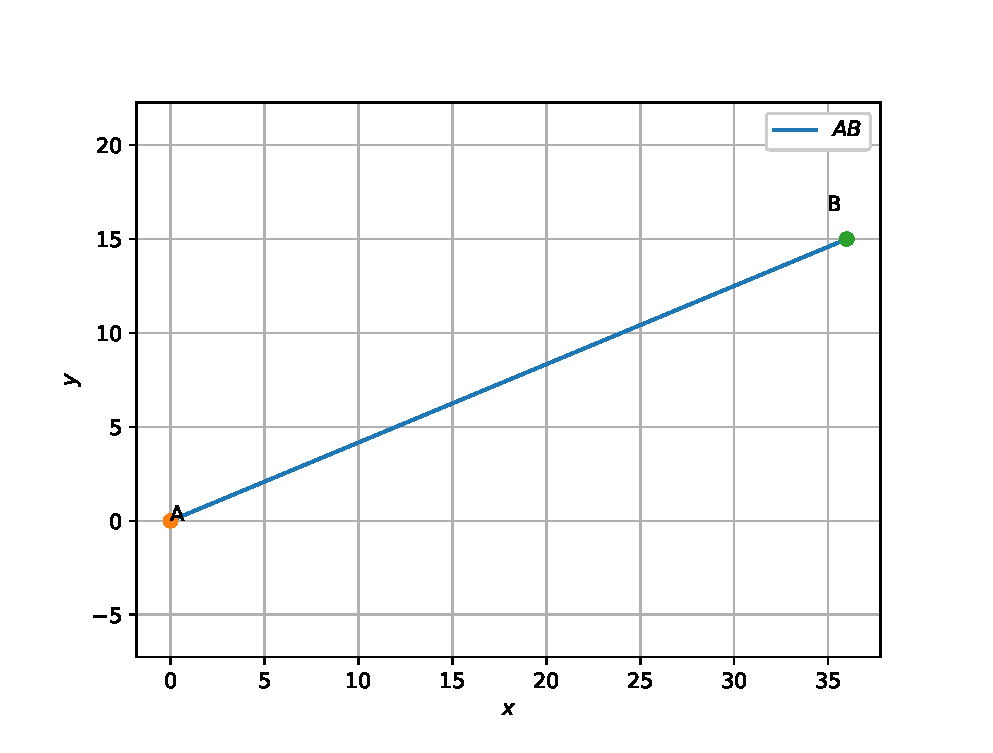
\includegraphics[width=\columnwidth]{./codes/line/towns/pyfigs/towns.eps}
\caption{Position of Towns A and B}
\label{fig:towns_py}
\end{figure}
So the distance between Town A and Town B is 39km.
\end{enumerate}
